\documentclass[linenumbers, twocolumn]{aastex631}


\newcommand{\vdag}{(v)^\dagger}
\newcommand\aastex{AAS\TeX}
\newcommand\latex{La\TeX}

\begin{document}

\title{The Milky Way and M31 Halo Remnant Shape}



\author[0000-0002-2527-8899]{Mika Lambert}
\affiliation{Steward Observatory and Department of Astronomy, University of Arizona, 933 N. Cherry Ave., Tucson, AZ 85721, USA}

\received{\today}

\keywords{Dark Matter Halo, Halo Shape, Cold Dark Matter Theory, Galaxy Merger, Merger Remnant }

%\begin{abstract}

%This example manuscript is intended to serve as a tutorial and template for authors to use when writing their own AAS Journal articles. The manuscript includes a history of \aastex\ and includes figure and table examples to illustrate these features. Information on features not explicitly mentioned in the article can be viewed in the manuscript comments or more extensive online documentation. Authors are welcome replace the text, tables, figures, and bibliography with their own and submit the resulting manuscript to the AAS Journals peer review system.  The first lesson in the tutorial is to remind authors that the AAS Journals, the Astrophysical Journal (ApJ), the Astrophysical Journal Letters (ApJL), the Astronomical Journal (AJ), and the Planetary Science Journal (PSJ) all have a 250 word limit for the abstract\footnote{Abstracts for Research Notes of the American Astronomical  Society (RNAAS) are limited to 150 words}.  If you exceed this length the Editorial office will ask you to shorten it. This abstract has 161 words.

%\end{abstract}

%% Keywords should appear after the \end{abstract} command. 
%% The AAS Journals now uses Unified Astronomy Thesaurus concepts:
%% https://astrothesaurus.org
%% You will be asked to selected these concepts during the submission process
%% but this old "keyword" functionality is maintained in case authors want
%% to include these concepts in their preprints.
%\keywords{Milky Way,  M31, Dark Matter Halo} 

\section{Introduction} \label{sec:intro}

% introduce topic
The two most massive bodies in the Local Group (LG) are the Milky Way (MW) and the Andromeda Galaxy (M31). The fate of these objects is an important part of understanding galaxy evolution and mergers because we can study their kinematics and mass profiles in great detail as they evolve. The interaction between these objects will also help us explore the cold dark matter paradigm. Since ... we believe these dark matter particles that weakly interact with baryonic matter make up $\sim$ 27\% of the matter in the universe \textbf{(ref)}. This dark matter forms complex structures in which galaxies reside. The mass profiles and shape of these dark matter halos around galaxies will shed light on their effect on the baryonic material. Major galaxy mergers, like the predicted merger between the MW and M31, are especially intriguing due to the multitude of dynamic processes occurring and the significant change in morphology of the merger remnant as a result. The merger remnant's halo may also have significant differences from the initial galaxies' halos as well.

% why the topic matters
Many simulations have been conducted predicting the motions of the MW and M31 and their course to a future collision \citep[e.g.,][]{2012VanDerMarel}.
%We propose investigating the characteristics of the dark matter halo remnant due to this future merger of the MW and M31. Using N-body simulations, we will explore the density profile of the halo remnant and the 3-dimensional shape of the halo. 

%\subsection{Why this topic matters to our understanding of galaxy evolution}
% what is a galaxy? and galaxy evolution
As M31 is the closest galaxy to the MW, our knowledge of that galaxy is greater than most other objects in the universe. Galaxy evolution, which is the process of changing the morphology and composition of galaxies \citep{2004galaxyevolutiondef}, is impossible to observe over human timescales, however, we can predict their evolution using N-body simulations.
N-body simulations of the merger event between the MW and M31 have accelerated our understanding of galactic merger events which have been hypothesized to be the source of the formation of high-mass elliptical galaxies. 
Understanding the profile of the halo remnant will further aid our quest to understand the behavior of cold dark matter because what categorically separates a galaxy from a star cluster is not being able to characterize its properties based solely on its baryonic matter \citep{2012Galaxydef}.
The resulting density profile from our experiment could also be compared to galaxies in more clustered environments that are believed to be the result of mergers which would shed light on the differences between mergers in the field versus in dense environments.
Further research could also be done on higher redshift galaxies (z $>$ 1) to look at early galaxy formation and merging.

%\subsection{Our current understanding of the topic}
According to \cite{2012VanDerMarel} the next major cosmic event to happen in the Local Group (LG) is the merger of the MW and M31 in $\sim$ 5 Gyrs. 
This event will not only change the physical shape of the baryonic matter of the LG, but also the dark matter halos of the galaxies.
We currently know that for equal-mass mergers, the shape of the halo remnant is dependent on the way the galaxies merge because the merger axis dictates the elongation shape, and the size of the remnant is related to the total energy of the merger \citep{2019drakos}. 
Another interesting aspect of the halos is the concentration of dark matter.
Modeling the density distribution of dark matter halos of galaxies is well defined by the Navarro-Frenk-White (NFW) profile \citep{1996NFW}. Visualizing the density profile of the halos using contour lines shows us the concentration of dark matter as seen in Figure \ref{fig:drakos}.
Astronomers also use simple relations between the mass of a galaxy's halo and its stellar mass using abundance matching \citep{2018Wechsler}. Abundance matching is the assumption that the halo mass is directly correlated to the stellar mass.
\begin{figure}[ht]
    \centering
    \includegraphics[scale=0.5]{drakos_fig_6.png}
    \caption{The density contours of the simulated remnant halos are in white, and the measured shape ratio is shown in red from \cite{2019drakos}. We see a clear difference in axis ratio between the two different panels.}
    \label{fig:drakos}
\end{figure}

%\subsection{Open questions in the field}
There are still many open questions within the realm of galaxy halo remnants.
More complex N-body simulations should be conducted accounting for the satellite galaxy's influence on the merging process. Also, the halos of dense galaxy clusters are still not well defined \citep{2019drakos}.
We can use these galaxy halos as laboratories for directly and indirectly detecting dark matter particles. An example of direct detection would be using our position in the MW to come across dark particles using facilities like LIGO, and indirect detection would search for the radiation produced by decaying dark matter particles \citep{2012Frenk_White}. In our own LG, the shape of the mass distribution of the merger remnant's halo would be an interesting question to pursue because we can apply our knowledge of this halo remnant to other galaxies and, in the future, build up statistics which could be used to predict the evolution of galaxy halos.
% include citations of current research being done

\begin{figure*}
    \centering
    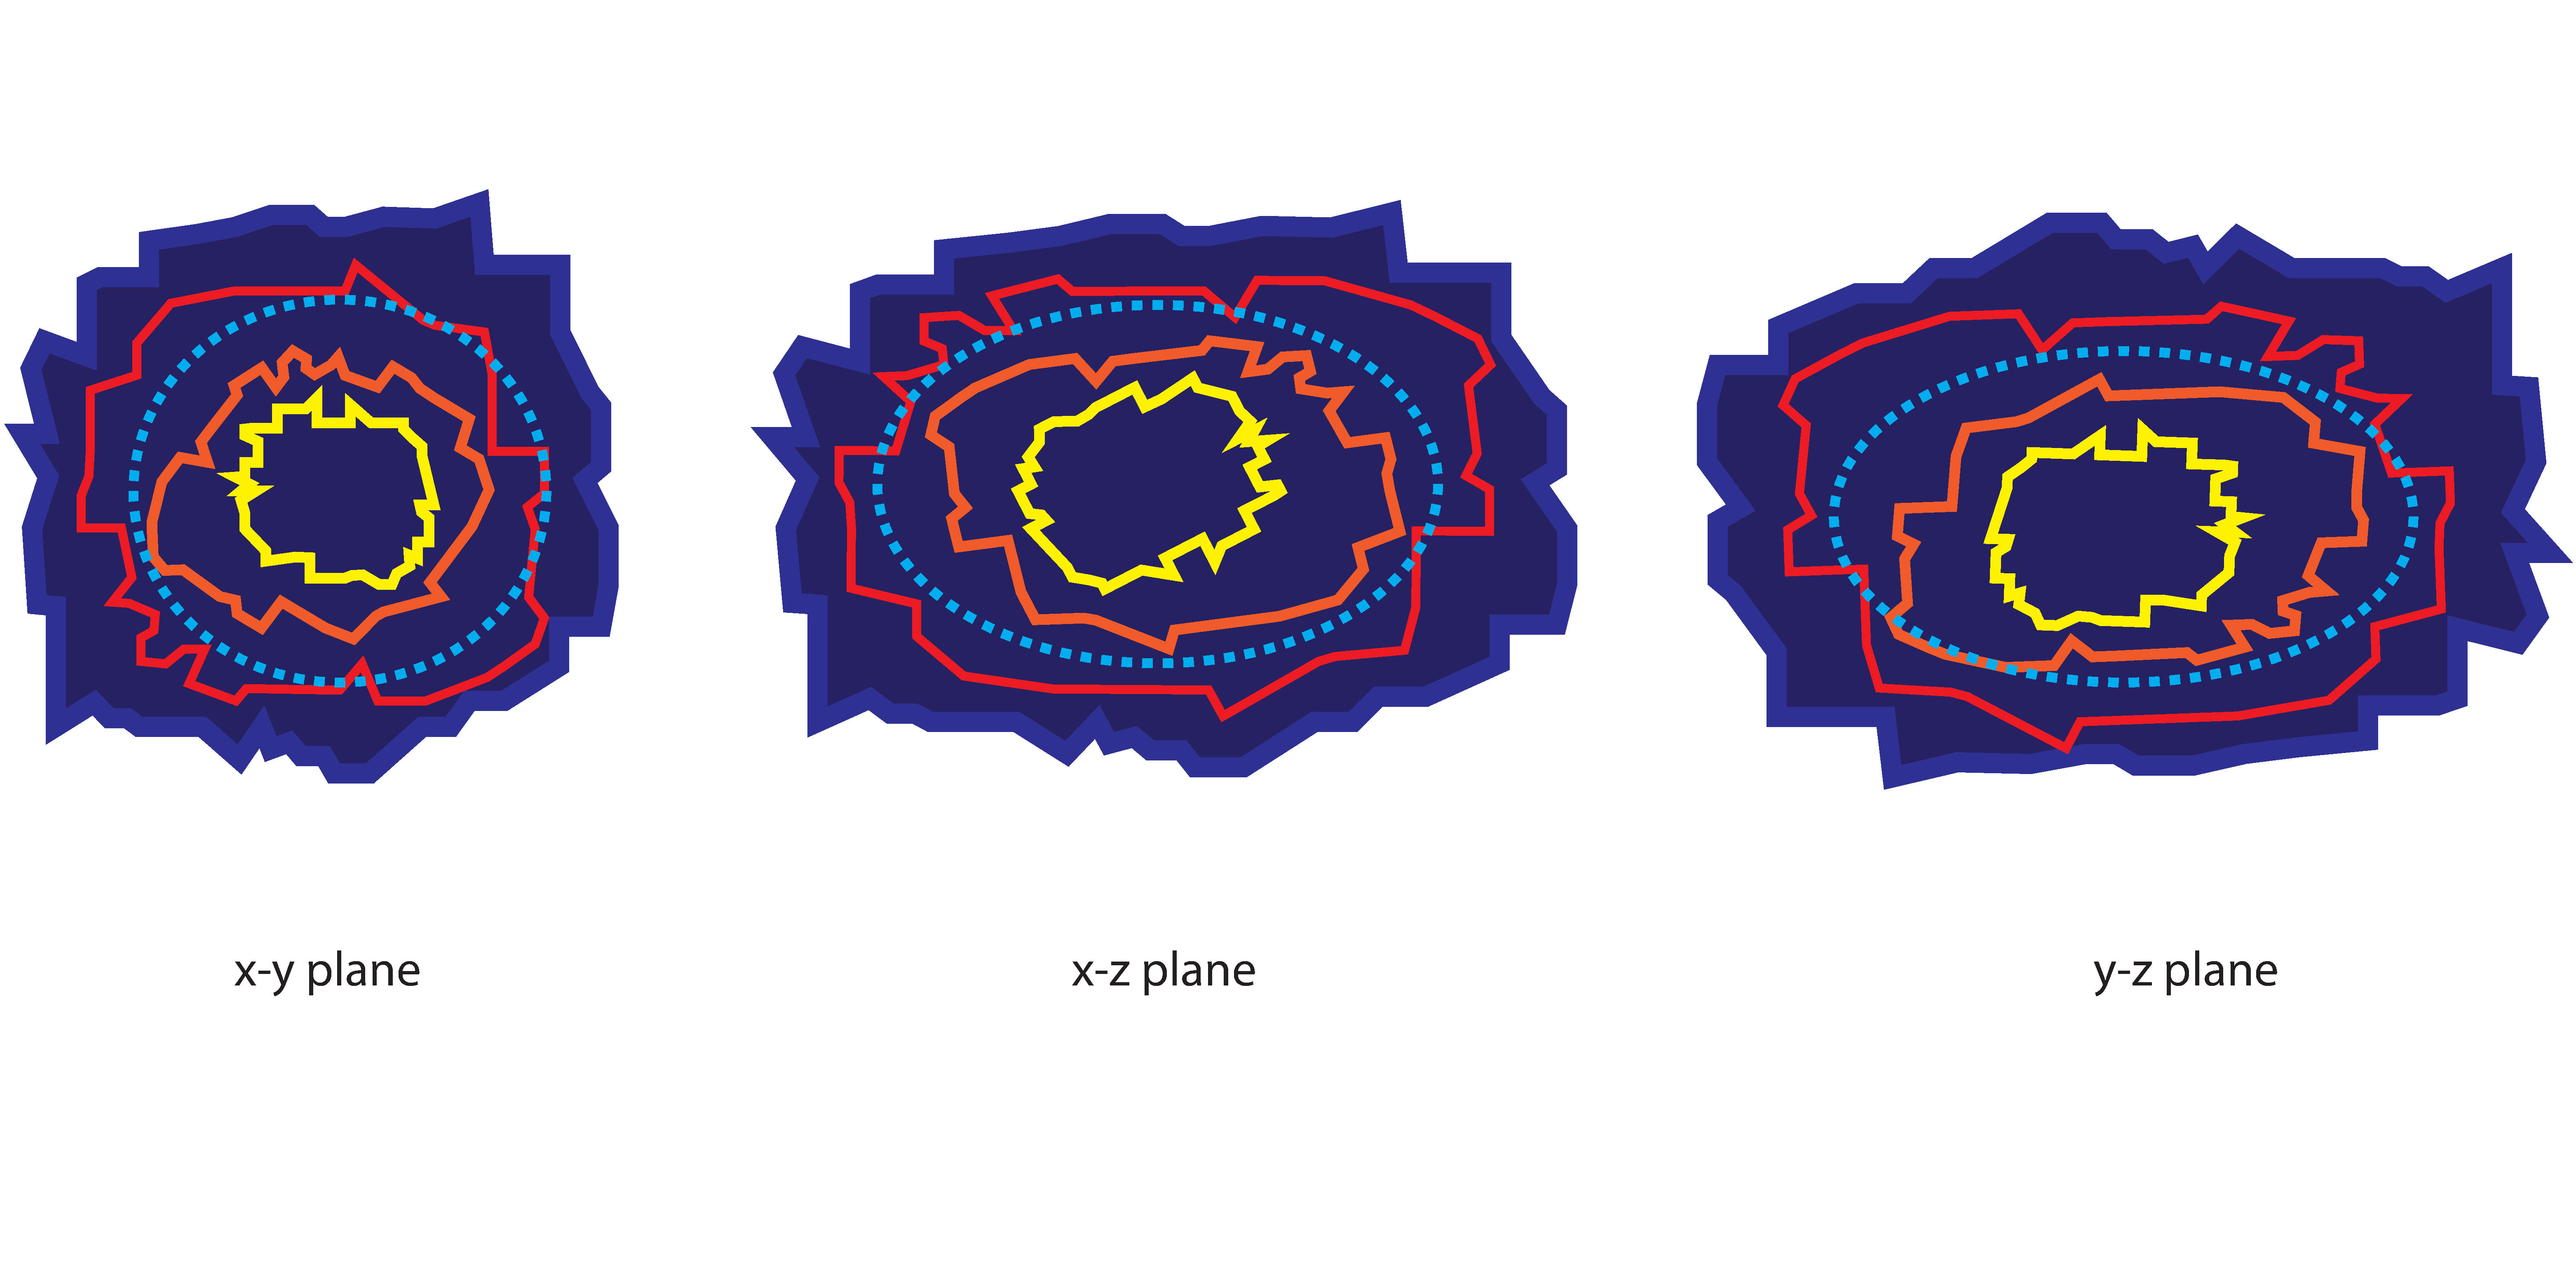
\includegraphics[width=\textwidth,height=10cm]{ASTR400B_proposal_diagram_2.pdf}
    \caption{The expected results from our methodology. Left: The halo remnant from the MW-M31 merger with density contours at 1$\sigma$ (yellow), 2$\sigma$ (orange), and 3$\sigma$ (red). The blue dashed line represents the ellipse with a projected axis ratio that appears to fit the halo distribution at the 2$\sigma$ isodensity contour. Middle: The x-z plane of the simulated halo remnant. Right: The y-z plane of the halo remnant with the same identifications as the other panels. We hypothesize that the halo will be triaxial so each axis ratio for each plane is different.}
    \label{fig:method_fig}
\end{figure*}

\section{This Project} \label{sec:project}

%\subsection{Questions} \label{sec:questions}
In this paper, we will be investigating the change in the 3-dimensional shape of the dark matter halo distribution from the MW halo to the MW and M31 merger remnant halo using the N-body simulation data from \cite{2012VanDerMarel}. 
Looking at the different axes of the distribution, We will determine whether the halo is spheroidal or elongated. 
We will describe the shape of the halo based on whether the shape is prolate, oblate, or triaxial which refers to the direction of flattening of the spheroidal objects.
We will quantitatively investigate the elliptical shape of the 2D projections of the halo in the three planes and characterize their semi-major and semi-minor axes by fitting ellipses to the 2$\sigma$ isodensity contour line.
%2. Is the 3D dark matter distribution spheroidal? or elongated like an ellipsoid? What do terms like prolate, oblate, or triaxial halos mean? https://astronomy.com/news/2010/ 01/astronomers-map-the-shape-of-galactic-dark-matter

%which question from above does this address
This will address the open question in the field that asks what is the mass distribution of the MW and M31 merger remnant's dark matter halo shaped like. The LG is a unique environment to be studying the halos of these objects because they are located in the field and both the MW and M31 are neither red and dead galaxies nor blue and star-forming galaxies. Being able to compare the MW and M31 halo remnant to dark matter halo simulations of galaxies of different colors and environments diversifies our understanding of halo evolution.


%why is this important for galaxy evolution? How will our study help address this open question?
Simulating the merger of these galaxy halos is important to galactic evolution as a whole because major mergers are essential to changes in galaxy morphology due to intense periods of star formation and inevitable quenching, yet it is still not fully understood what happens to the dark matter particles during a merger. Examining the physical shape of the dark matter halo remnant may open avenues to look into probing why the remnant is the shape it is, how dark matter interacts with itself, and if it correlates to the baryonic matter. Similar to how the galactic morphology of the baryonic matter is visually classified, we may start to see a pattern of simulated halos that we can categorize.


\section{Methodology} \label{sec:methodology}

% introduce the N-body simulations
The N-body simulation used in this study is from \cite{2012VanDerMarel}. They considered only stars and dark matter particles that were collisionless and used the hydrodynamic code, GADGET-3 \cite{}. The simulation does not account for gas since it is only a small fraction of the total mass of the galaxy. This also allows for more star and dark matter particles and the simulations are at high resolution for those characteristics. The simulation begins at the current epoch and has 800 snapshots. Each snapshot corresponds to the following relation to calculate the time: Snapshot$*10/.7$ = time (Myrs).

In order to characterize the shape of the halo remnant we use the following approach.
First, we will need to probe the shape of the spatial mass distribution of the MW halo at snapshot 0 using a 2D histogram along all three axes to investigate any non-spheroidal attributes it may have. To do this, we will implement the code from Lab 7 to create the density contours, and we will also need to rotate the position vectors so that the halo's angular momentum is aligned with the z-axis. We will look at the x-y plane, the x-z plane, and the y-z plane distributions for any elongation. Using an ellipse function to fit the contour lines, and we will calculate the semi-major and semi-minor axes. We will also use visual checks to confirm the ellipse is a reasonable  estimate of the contour line.
We will do a similar procedure for the MW-M31 halo remnant using snapshot 700 using a 2D histogram along the three axes and look for prolate or oblate features by looking at the x-y plane, the x-z plane, and the y-z plane. We use snapshot 700 because a snapshot value of 700 gives a time of 10Gyrs. This is where we define the merging galaxies to be relaxed dynamically, and the stars from the MW and M31 are well mixed according to \cite{2012VanDerMarel}. If only one of the planes shows elongation, we will assume the shape is more oblate. If two of the planes show elongation, we will assume the distribution is more prolate. If all three planes are relatively circular, then we will assume the halo remnant distribution is spheroidal. If we see that the axes are different in all three planes we will assume the shape is triaxial. We will also estimate the ellipsoidal measurement of the semi-major and semi-minor axes for the remnant.
The density contours seen in Figure \ref{fig:method_fig} show how concentrated the mass of the halo is. The blue line is the estimated projected ellipse for the corresponding plane. We will use visual checks to determine what the estimated axis ratio is.


We will create an additional function that creates an ellipse with $\tt{matplotlib}$ using the 2$\sigma$ contour as a reference for comparing snapshot 0 to 700 to be consistent at the same density. This function will also calculate the semi-major and semi-minor axes which will give us quantitative measurements of the shape of the halo. First we calculate the covariance of the two coordinates, then we normalize them which gives us the Pearson Correlation Coefficient. Lastly, we can calculate the horizontal and vertical radius using $sqrt(1+p)$ and $sqrt(1-p)$ respectively and divide by 2 times the desired sigma level. Then, we can plot the ellipse with these given parameters.
To track the evolution of the axis ratio we will need to loop over this ellipse function for each plane and every tenth snapshot.


%plots:
%- contour plots for snapshot 0 and snapshot 700
%- plot axis ratio with time for 
%- If time permits, find if the axis of elongation would be in the direction of relative motion between the galaxies.

We will first be creating plots similar to \ref{fig:method_fig}. We will have two sets of subplots, one at snapshot 0 in the x-y, x-z, and y-z planes with the modeled ellipse overlaid, and at snapshot 700 in the x-y, x-z, and y-z planes with the modeled ellipse overlaid to determine their axis ratio. We will also create a plot of the evolution of the axis ratio in each of the three planes over time from snapshot 0 to 700. We will use every 10 snapshots to get a general sense of how the halo shape evolves with time. This halo shape will focus on the MW particles because adding the additional particles of M31 is beyond the scope of this study. Theoretically, if one were to include M31's particles to this axis ratio evolution plot, they would need to consider the point in time where they can say M31 and the MW particles are well mixed which would not occur until snapshot 700 based off of our assumptions.


%\subsection{Hypothesis} \label{sec:hypothesis}
As seen in Figure \ref{fig:drakos} for the merger between two equal-mass galaxies, we would expect a similar shape to emerge from the halo of the MW-M31 halo remnant which is more triaxial than spheroidal with one long axis and two short axes as seen in Figure \ref{fig:method_fig}. 
%This makes sense due to the momentum the collision transfers and we would expect the axis of elongation would be in the direction of relative motion between the galaxies.
Prolateness also depends on the amount of mass loss, so in the future, one can use our result to estimate the amount of mass that would no longer be under the gravitational effects of the remnant.
We also expect the axis ratio to become less symmetric over time as the merger happens.


\bibliography{sample631}{}
\bibliographystyle{aasjournal}

%% This command is needed to show the entire author+affiliation list when
%% the collaboration and author truncation commands are used.  It has to
%% go at the end of the manuscript.
%\allauthors

%% Include this line if you are using the \added, \replaced, \deleted
%% commands to see a summary list of all changes at the end of the article.
%\listofchanges

\end{document}

% End of file `sample631.tex'.
